% Scene B of "Render a ping without Gazebo" (render-a-ping.md), from gz_sonar/examples/render_ping.cc:
% imaging sonar (ECHO, 20 deg tall, 10 m window) 2 m above a flat seabed, pitched down 15 deg; a 1 x 1 x 0.5 m box
% from 4.5 to 5.5 m ahead. The lower beam edge (25 deg down) meets the seabed at 4.29 m (4.73 m slant); the box's far
% top edge shadows the seabed out to 5.5 * 2 / 1.5 = 7.33 m. Side view, true scale, 1 unit = 1 m.
% Build: pdflatex render_ping_B.tex, then pdftocairo to ../images/render_ping_B.{png,svg}
\documentclass[tikz,border=6pt]{standalone}
\usetikzlibrary{arrows.meta,calc}
\renewcommand{\familydefault}{\sfdefault}
\tikzset{
  lbl/.style={font=\sffamily\small},
  beam/.style={fill=black!7,draw=black,thin},
  dim/.style={thin,{Latex[length=1.6mm]}-{Latex[length=1.6mm]}},
  lead/.style={thin,black!70},
  axis/.style={thin,dashed},
  shadow/.style={fill=black!30,draw=none},
}
% seabed line from x0 to x1 at height z (drawing units), slab of dots below
\newcommand{\seabed}[3]{
  \draw[thick] (#1,#3) -- (#2,#3);
  \foreach \r [count=\i] in {0.12,0.3} {
    \pgfmathsetmacro{\o}{mod(\i,2)*0.12}
    \pgfmathsetmacro{\n}{int((#2-#1-0.3)/0.24)}
    \foreach \k in {0,...,\n} \fill ({#1+0.12+\k*0.24+\o},{#3-\r}) circle (0.4pt);
  }
}
% sonar head at #1, pitched down #2 degrees
\newcommand{\head}[2]{
  \begin{scope}[shift={#1},rotate=-#2]
    \draw[fill=black!15] (-0.5,-0.13) rectangle (0,0.13);
    \fill (0,0) circle (1.4pt);
  \end{scope}
}
\begin{document}
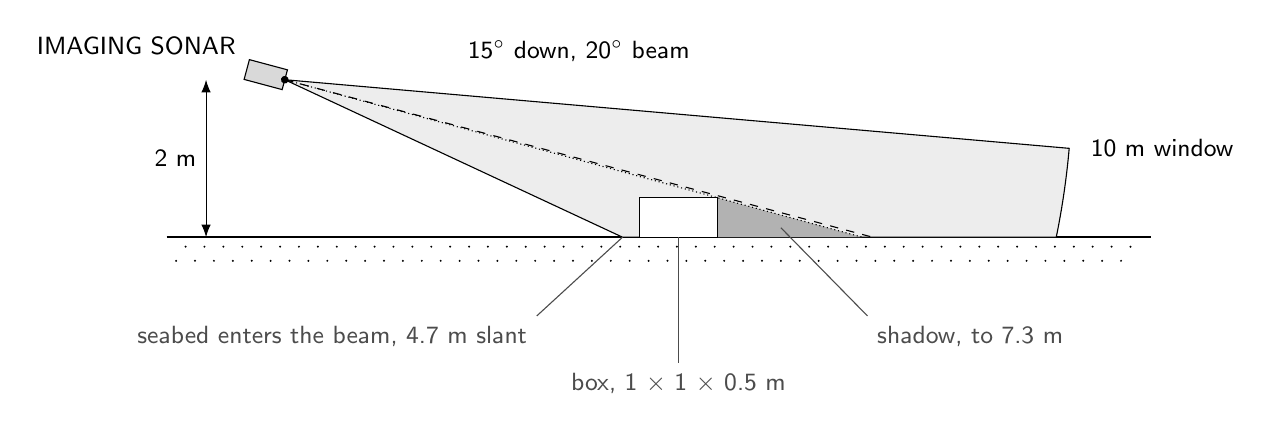
\begin{tikzpicture}[scale=1.0]
  \pgfmathsetmacro{\xn}{2/tan(25)}          % lower edge meets the seabed
  \pgfmathsetmacro{\xf}{sqrt(100-4)}        % 10 m window meets the seabed
  \pgfmathsetmacro{\af}{asin(0.2)}
  \seabed{-1.5}{11}{0}
  \draw[beam] (0,2) -- ({10*cos(5)},{2-10*sin(5)}) arc (-5:-\af:10) -- (\xn,0) -- cycle;
  \draw[axis] (0,2) -- ({2/tan(15)},0);
  % shadow behind the box
  \fill[shadow] (5.5,0.5) -- (7.333,0) -- (5.5,0) -- cycle;
  \draw[thin,densely dotted] (0,2) -- (7.333,0);
  \draw[fill=white] (4.5,0) rectangle (5.5,0.5);
  \head{(0,2)}{15}
  % dimensions and labels
  \draw[dim] (-1,2) -- (-1,0) node[lbl,midway,left] {2 m};
  \node[lbl,anchor=west] at ({10*cos(5)+0.15},{2-10*sin(5)}) {10 m window};
  \node[lbl,anchor=south west] at (2.2,2.1) {15$^\circ$ down, 20$^\circ$ beam};
  \draw[lead] (\xn,0) -- (3.2,-1.0) node[lbl,anchor=north east] {seabed enters the beam, 4.7 m slant};
  \draw[lead] (5,0) -- (5,-1.6) node[lbl,anchor=north] {box, 1 $\times$ 1 $\times$ 0.5 m};
  \draw[lead] (6.3,0.12) -- (7.4,-1.0) node[lbl,anchor=north west] {shadow, to 7.3 m};
  \node[lbl,anchor=south east] at (-0.5,2.2) {IMAGING SONAR};
\end{tikzpicture}
\end{document}
